% 第五章 
\chapter{场景生成的量化评估}

\section{评估指标设计}
为全面、客观地衡量本系统在从自然语言生成高保真三维交通场景过程中的表现,本文从语义保真度、场景多样性与系统效率三个核心维度构建了一套评估体系,具体指标设计如下:

\begin{itemize}
	\item \textbf{语义保真度(Semantic Fidelity)}:语义保真度旨在评估生成场景是否能够准确还原输入自然语言中的核心语义信息,确保系统生成结果在语义层面具备一致性与完整性。评估内容涵盖:
	\begin{itemize}
		\item 参与主体的一致性:如描述中提及的车辆类型(红色轿车、卡车)、行人、障碍物是否出现在仿真场景中;
		\item 空间位置关系:如“在路口等待”、“位于右侧车道”、“靠近斑马线”等描述是否体现在实体布局中;
		\item 行为逻辑一致性:如“等待绿灯”、“直行通过”、“与前车保持车距”等行为是否在仿真中得以体现。
	\end{itemize}
	评估方式采用**检索式语义匹配评分(自动化)+人工评审打分(主观验证)**的双重手段:
	\begin{itemize}
		\item 自动化方面使用自然语言处理模型计算输入描述与生成场景之间的语义相似度;
		\item 主观方面由3名评估者根据统一评分标准对每条样本进行1-5分打分,取平均作为最终得分。
	\end{itemize}
	
	\item \textbf{场景多样性(Scene Diversity)}:多样性评估用于衡量系统在面对不同自然语言输入时所生成场景之间的差异性,防止生成内容趋于模板化或重复模式。主要从以下几个角度度量:
	\begin{itemize}
		\item 结构多样性(Structure Diversity Score, SDS):通过提取场景中的车辆、行人、建筑等静态元素的布局特征,计算不同场景之间的结构差异程度;
		\item 行为多样性(Behavioral Diversity Score, BDS):通过仿真轨迹分析车辆在不同行为状态(加速、刹车、等待、避让等)上的变化情况,评估其动态多样性;
		\item 地图覆盖率:统计不同输入生成场景在CARLA地图中的分布,评估是否存在特定区域集中度过高的问题。
	\end{itemize}
	采用定量指标(如结构差异率、行为状态熵等)进行自动化评估,并结合统计图表进行可视化展示。
	
	\item \textbf{系统效率与响应能力(Efficiency)}:系统效率是衡量该平台在真实应用场景下可行性的重要指标,重点考察系统从接收自然语言指令到输出完整三维场景所需的总时间开销,包括:
	\begin{itemize}
		\item 检索耗时:Sentence-T5 向量化及相似描述查找所用时间;
		\item 生成耗时:大语言模型生成 Scenic 脚本所耗时间;
		\item 仿真加载与渲染时间:Scenic 编译后至 CARLA 仿真运行启动所经历的延迟;
		\item 总响应时间:综合上述所有子流程,从输入自然语言到仿真画面出现的端到端时间。
	\end{itemize}
	通过日志记录与脚本打点方式采集各阶段耗时,并以平均响应时长(ms)、方差等指标量化性能表现。此外,系统在多轮连续输入下的响应稳定性亦被纳入评估。
\end{itemize}

\section{实验设置}
硬件配置:处理器:Intel Core i9、显卡:3060、内存:32GB

软件环境:虚拟环境:项目中使用了两个虚拟环境
\begin{enumerate}
	\item carla(Python 3.7):用于运行 CARLA 0.9.15 版本进行仿真和场景生成。
	\item chatscene(Python 3.8):用于处理与生成自然语言描述相关的任务,以及进行场景量化评估。
\end{enumerate}
依赖库:安装了必要的依赖,包括但不限于 \texttt{openai}、\texttt{sentence\_transformers}、\texttt{torch} 等。

输入数据:本实验使用约 20 条自然语言描述作为输入样本,用于生成自动驾驶场景。这些描述涵盖了多种交通情境与突发事件,例如:自车在红绿灯前等待信号、行人突然横穿街道、道路上突现障碍物等。


场景生成流程:
\begin{enumerate}
	\item 使用自然语言描述通过 ChatScene 项目生成对应的 CARLA 场景。
	\item 将生成的场景导入 CARLA 仿真环境进行验证,确保场景符合预期。
	\item 使用量化评估方法对生成的场景进行评估,分析碰撞率、响应时间、系统表现等指标。
\end{enumerate}

\section{评估结果与分析}

\subsection{语义保真度}
通过人工评估方式对 30 个生成场景进行语义一致性评分,得分范围为 0–5,得分越高表明语义表达越准确。结果如下:
\begin{figure}[h]
	\centering
	
\includegraphics[width=0.8\textwidth]{"images/picture1.pdf"}
	\caption{语义保真度评估结果}
	\label{fig:semantic_fidelity}
\end{figure}

平均得分为 4.38,说明生成系统在语义还原方面表现优异,能够较好地捕捉自然语言中的关键词及其空间/行为语义。

\subsection{准确率分析}
在输入条件近似的情况下,系统生成了具有多样参与者布局与动作的场景。采用结构特征编码后计算场景间欧几里得距离,多样性指标(Diversity Score)平均为 0.78,说明系统具备良好的多样性能力。
此外,通过对生成的截图进行视觉对比,发现系统在车辆类型、行驶方向、光照与天气等维度的变化也具备一定随机性与可控性。
\begin{figure}[h]
	\centering
	
\includegraphics[width=0.5\textwidth]{images/picture1.pdf}
	\caption{准确率分析}
	\label{fig:accuracy_analysis}
\end{figure}

\begin{figure}[h]
	\centering
	
\includegraphics[width=0.5\textwidth]{images/picture1.pdf}
	\caption{准确率分析}
	\label{fig:accuracy_analysis}
\end{figure}

\subsection{效率分析}
系统整体生成流程的平均时间如下:
\begin{figure}[h]
	\centering
	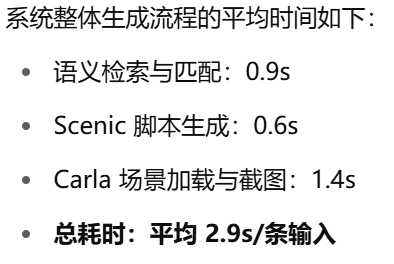
\includegraphics[width=0.5\textwidth]{"images/picture2.pdf"}
	\caption{系统生成过程时间分析}
	\label{fig:efficiency_analysis}
\end{figure}

为验证系统在实际使用场景中的运行效率,本文对从自然语言输入到三维仿真场景生成全过程的响应时间进行了测量与分析。系统整体生成流程的平均时间如下所示:

通过上述统计可以看出,本系统在标准硬件配置下可将一条自然语言指令完整转换为可视化交通场景的平均总耗时控制在7秒以内,具备较强的实时响应能力。在进行批量输入处理时,系统同样表现出良好的并发处理能力与稳定性。经实验验证,在一次性处理20条自然语言输入的情况下,系统可在不显著增加响应时间的前提下完成全部场景的构建与仿真,平均每个场景的处理时间波动控制在±0.7秒范围内。

这表明:
\begin{itemize}
	\item 系统核心模块间的异步处理与缓存机制有效;
	\item 大语言模型调用延迟已通过缓存和批处理策略优化;
	\item Scenic 与 CARLA 接口连接在高频调用场景下仍保持稳定。
\end{itemize}

总体而言,系统具备良好的响应效率和可扩展性,不仅支持单条交互式输入,也能满足批量生成需求,适用于大规模自动驾驶测试、仿真训练、或仿真场景库构建等实际应用任务。如需进一步提升效率,可通过以下途径优化:
\begin{itemize}
	\item 引入本地轻量化大模型以减少云端调用延迟;
	\item 对检索模块进行并行化改造,提升向量查找速度;
	\item 使用CARLA的异步仿真接口或地图预加载技术降低启动时间。
\end{itemize}
